\section*{Introduction}

Pour la mise en œuvre de notre travail nous avons opté pour l'utilisation d'Apache Cassandra, qui est une base de données NoSQL à colonnes larges bien établie. Il utilise un modèle de stockage basé sur des colonnes pour capturer de grandes quantités de données non structurées.

Cassandra se concentre sur le fonctionnement d'un cluster distribué de serveurs de base et bénéficie d'une haute disponibilité et d'une mise à l'échelle horizontale flexible.

Tout au long de cette partie nous présenterons les étapes d'installation de ces technologies ainsi que les outils de développement utilisés pour développer un simulateur qui génère des données pour la gestion d'électricité dans le cadre d'un smart grid.

\begin{figure}[h]
	\centering
    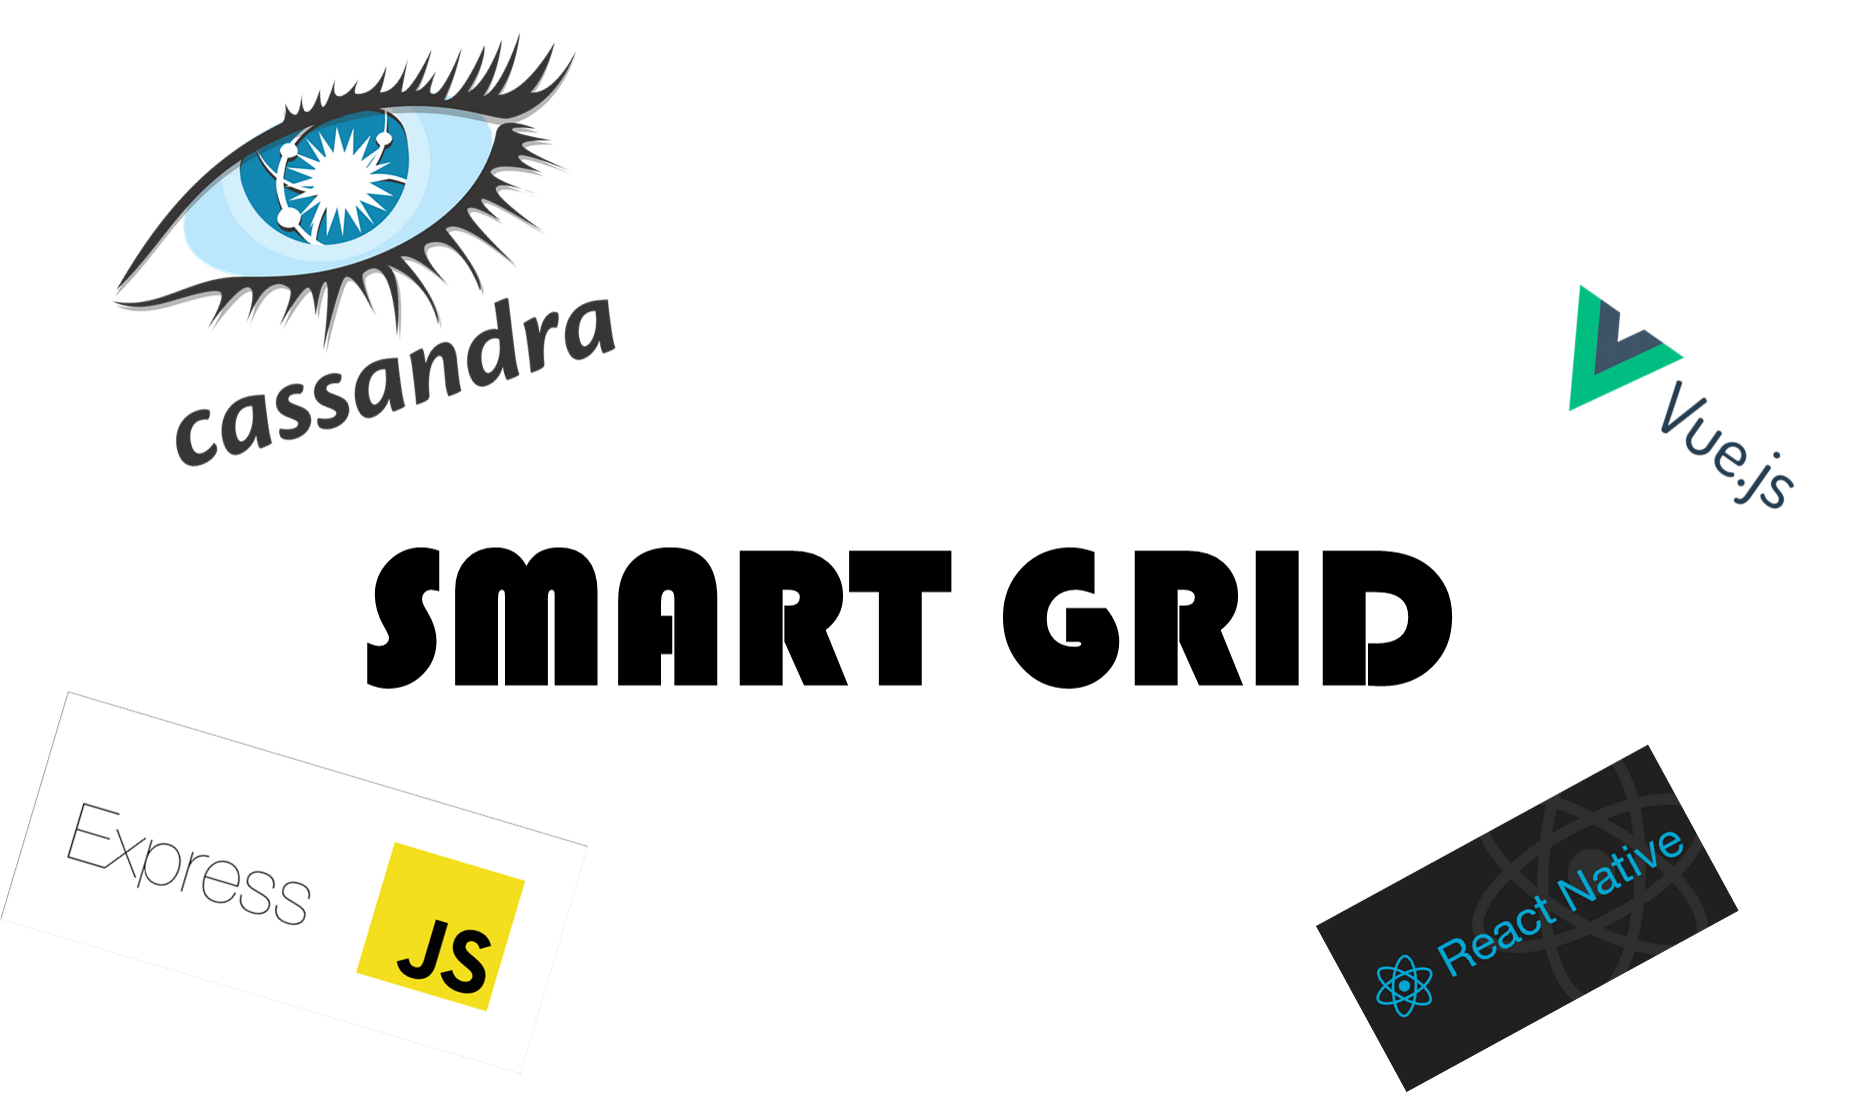
\includegraphics[scale=0.5]{img/part3/1.1}
    \caption{Technologies utilisé}
\end{figure}
